\section{Case Study}
\label{sec:case}

\begin{figure}[t]
\begin{scriptsize}
%\begin{verbatim}
\begin{lstlisting}
declare
def accumulate
	cart_action <= action_msg.map { |c| [c.session, c.item, c.action, c.reqid] }
	action_cnt <= cart_action.group([cart_action.session, cart_action.item, cart_action.action], count(cart_action.reqid))
end

declare
def summarize
	status <= join(action_cnt, checkout_msg).map do |a, c|
		if a.action == "Add" and not action_cnt.map{|d| d.id if d.action == "Del"}.include? a.id 
			[a.session, a.item, a.cnt] 
		end 
	end

	status <= join([action_cnt, action_cnt, checkout_msg]).map do |a1, a2, c| 
		if a1.session == a2.session and a1.item == a2.item and a1.session == c.session and a1.action == "Add" and a2.action == "Del"
			[a1.session, a1.item, a1.cnt - a2.cnt] if (a1.cnt - a2.cnt) > 0
		end
	end
end

declare 
def communicate
	response_msg <+ join([status, checkout_msg]).map do |s, c| 
		if s.session == c.session
			[c.client, c.server, s.session, s.item, s.cnt]
		end
	end

	action_msg <+ join([action_msg, member]).map do |a, m|
		unless member.map{|nm| nm.player}.include? a.client
			[m.player, a.server, a.session, a.item, a.action, a.reqid]
		end 
	end
end
\end{lstlisting}
%\end{verbatim}
\vspace{-10pt}
\caption{Disorderly cart implementation.}
\label{fig:pdg-disorderly}
\end{scriptsize}
\vspace{-2pt}
\end{figure}

%%\wrm{Re-do case studies in Bud} \wrm{Break cart development down into
%%iterations} \wrm{How does the language naturally lead us to an order
%%independent style?  Talk about inserting all sorts of exotic stuff like queues
%%if we want a highly order-dependent imperative style.}

\begin{comment}

\jmh{We discussed the following on the phone.  (1) Handle shopping in two styles: destructive updates, and disorderly accumulation of increment/decrement.  (2) Do analysis on them to detect need for coordination in only the first, show that (annotated) 2PC removes the compiler warning.  (3) Deploy destructive+2PC on EC2 and show practical benefits of avoiding coordination.  (4) Evolve the program with new rules for checkout and/or inventory, show how the disorderly version is no longer monotonic.  Fix that  with 2PC where needed.  Also make sure the destructive version works with the new rules.  Now show that the disorderly version is still better than the destructive one, by coordinating only where needed.}

\jmh{Finally, show what would happen if you didn't coordinate the inventory bit, but tracked taint.  Note that tainted output is the stuff where programmers need to write compensation logic.}

\end{comment}

In this section, we develop two different designs for a distributed shopping-cart
application in Bloom.  First, we implement a ``destructive,'' state-modifying
shopping cart application using a simple key-value store (also written in Bloom).
Second, we implement a ``disorderly'' cart that accumulates updates in a 
set-wise fashion, summing up the updates at checkout into a final result.  These two different designs illustrate our analysis tools and the way they inform design decisions for distributed programming.

We begin with a shopping cart built on a key-value storage abstraction.  Each
cart is a \texttt{(key,value)} pair, where \texttt{key} is a unique session
identifier and \texttt{value} is an object containing the session's state,
including a Ruby array that holds the items in the cart. Adding or deleting
items from the cart result in ``destructive'' updates: the value associated with
the key is replaced by a new value that reflects the effect of the
update. Deletion requests are ignored if the item they refer to does not exist
in the cart.

Figure~\ref{fig:pdg-destructive} shows the Bloom code for this design.  The
\textbf{scratch} \texttt{kvput} is defined by the \texttt{KeyValueStore} module (10
lines of Bloom not shown here), which the shopping cart extends via
inheritance; it represents the input interface to the key-value store.
%; it is used in a manner analogous to the \emph{put} function for hash tables.  
The set of shopping carts is represented by the persistent \textbf{table} \texttt{bigtable}, which is replicated
%%The \texttt{bigtable} replicas are kept consistent 
by shipping \texttt{kvput} tuples between replicas upon updates. 
%%\wrm{this doesn't guarantee consistency... might be better to say "bigtable is replicated..."}.
% Ideally, when all messages have been delivered, every server should have an 
% identical copy of \texttt{bigtable}.

%%\paa{TODO:}\jmh{Any reason not to move line 28 to the top and reference it here?}
In line 27, the client transmits \texttt{client\_action} tuples that correspond to cart
updates over the \texttt{action\_msg} \textbf{channel} to an individually
chosen server replica.  We assume that the client has already chosen a server
based on load balancing.
%\jmh{say how chosen.}
%\jmh{which server replica?  all server replicas??} 
For each such arriving
tuple, line 3
checks \texttt{bigtable} to see if a record exists for the
session associated with the \texttt{action\_msg}.  If none is there (i.e., this
is the first update for a new session), then lines 4--8 generate an entry for
the new session in \texttt{bigtable}.  Otherwise, the join conditions in lines 12--13 are
satisfied and lines 14--20 ``replace'' the item array
at the next timestep with a new version.  
%\jmh{lines 15 and 16 do not fit my definition of Bloom above.  Not sure how to deal with that.} %\jmh{I added a note above that we allow simple side-effect-free Ruby expressions.}
Whenever a \texttt{checkout\_msg} appears in a server replica, the 
\texttt{bigtable} tuple associated with the given session is identified (via the join
on lines 29--30), and the item array in its value field is sent back to the client.  

%\jmh{Note that checkout is idempotent because checkout\_msg is a persisted set?}

Figure~\ref{fig:pdg-disorderly} shows an alternative shopping cart implementation, in which
updates are monotonically accumulated during shopping in a disorderly set, and summed up
only at checkout.  Line 3 inserts all client updates into the persistent table
\texttt{cart\_action}.  Lines 4--5 define \texttt{action\_cnt} as an aggregate
over \texttt{cart\_action}, in the style of an SQL \texttt{GROUP BY} statement: for each
item associated with a cart, we separately count the number of times it was
added and the number of times it was deleted.   
%Lines 5--16 define the collection
%\texttt{status} as the union of the session, item and action fields resulting from 
%a 3-way join between the \texttt{checkout} message and two
%copies of \texttt{action\_cnt}---one corresponding to additions and one to
%deletions -- and the set of \texttt{action\_cnt}  tuples corresponding to items 
%for which there is no deletion in a given session.
Lines 11--16 ensure that when a \texttt{checkout\_msg} tuple arrives, \texttt{status} 
contains a record for every added item
for which there was no corresponding deletion in the session.  Lines 18--23 
additionally define \texttt{status} as the 3-way join of the \texttt{checkout\_msg}
message and two copies of \texttt{action\_cnt}---one corresponding to additions and one to
deletions.
Thus, for each item, \texttt{status} contains its final quantity: the
difference between its number of additions and deletions (line 21), or simply the number
of additions if there are no deletions (line 14). 
Upon the appearance of a \texttt{checkout\_msg}, the
replica returns a \texttt{response} message to the client containing the
final quantity (lines 28--32).  
Because the disorderly implementation does not use a separate
storage system, it includes its own logic for state replication (lines 34--38).
Line 36 ensures that only the replica contacted by the client performs a multicast,
by probing the \textbf{table} \texttt{member} to see if the \texttt{action\_msg} 
originated inside the quorum.

\begin{figure}[t]
\centering
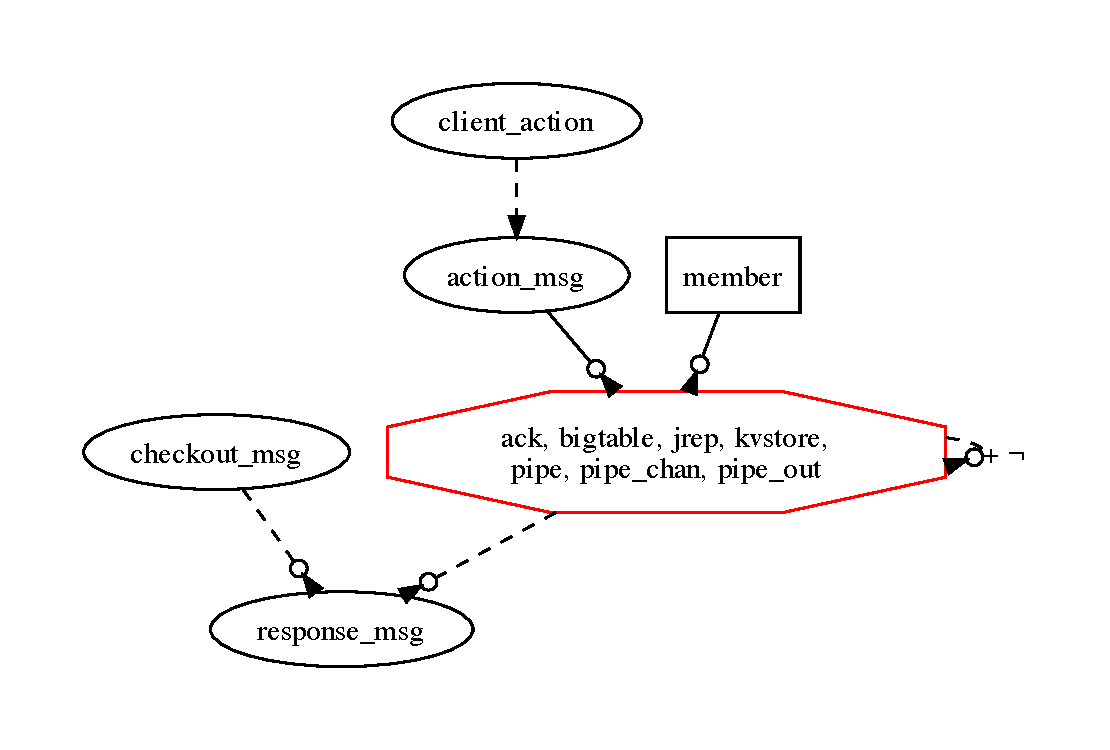
\includegraphics[width=0.9\linewidth]{fig/destructive.pdf}
\vspace{-10pt}
\caption{Destructive cart analysis.}
\label{fig:pdg-destructive-analysis}
\vspace{-2pt}
\end{figure}

\begin{figure}[t]
\centering
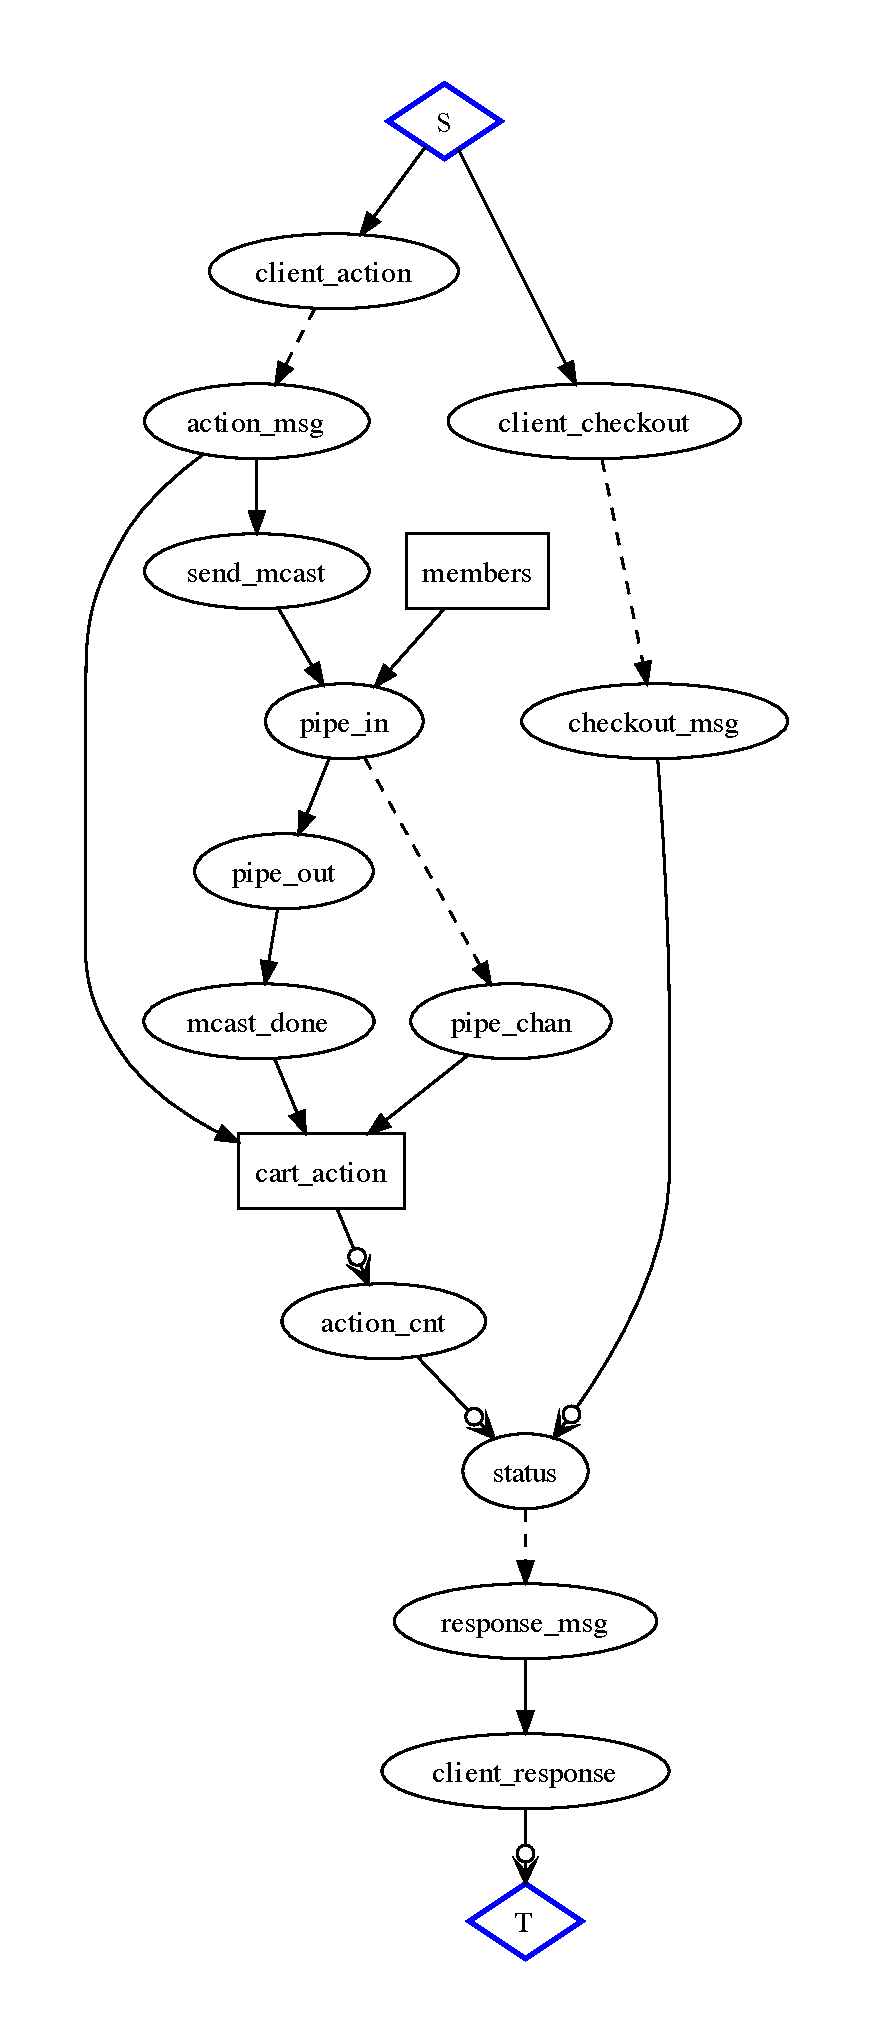
\includegraphics[width=0.7\linewidth]{fig/disorderly.pdf}
\vspace{-10pt}
\caption{Disorderly cart analysis.}
\label{fig:pdg-disorderly-analysis}
\vspace{-2pt}
\end{figure}

%%\jmh{need an explanation of lines 5-9, or an alternative syntax (see below or implement LOJ).  %%In the last sentence do you mean lines 24-30?  Won't 28-30 result in each node multicasting %%checkouts to each other node, i.e. $n^2$ messages?}

%\subsection{Analysis}
\noindent
\textbf{Analysis}\\
\noindent
%For each cart, we apply whole-program analysis techniques to discover points
%of order.
The Bud interpreter automatically generates a graphical
representation of dependencies between collections in a program
(Figures~\ref{fig:pdg-destructive-analysis} and \ref{fig:pdg-disorderly-analysis}).
%The Bud interpreter automatically generates a graphical representation of the
%dependency graph of collections through rules, (and hence the flow of tuples)
%as a staged dataflow.
Each node in the graph is either a collection or a cluster of collections; \textbf{table}s are shown as rectangles, ephemeral
collections (\textbf{scratch} and \textbf{channel}) are depicted as ovals, and clusters (described below) as octagons.  A
directed edge from node $A$ to node $B$ indicates that $B$ appears in the
lhs of a Bloom rule with $A$ referenced directly, or through a join expression,
in the rhs.  An edge is annotated based on the operator symbol in the rule and
the type of $B$.  If the rule is ``inductive''---i.e., has the \texttt{$<$+}
operator and a {\bf table} lhs---then the edge is marked with a $+$.  If the
rule is ``asynchronous''---i.e., a rule with the \texttt{$<$+} operator and a {\bf
channel} lhs---then the edge is a dashed line.  If the rule involves
non-monotonicity (aggregation or negation) over $A$, then the edge is marked with a $\lnot$.
%result in edges marked with a $\lnot$.
To make the visualizations more readable, any strongly connected component with both a $\lnot$ and a $+$ edge is collapsed into a octagonal ``temporal cluster,'' 
which can be viewed abstractly as a single, nonmonotonic node in the 
dataflow.\footnote{Datalog aficionados may be troubled by our mention of cycles
involving negation in the dependency graph.  In~\cite{dedalus-techr} we
describe why the inclusion of a $+$ edge in such a cycle ensures stratifiability.}
%\jmh{capturing what? the fact that they must recurse over multiple timesteps? we can't just intro %this without any intuition.  You should also dismiss the particular collection names in this 
%figure as details from the KV store that are beyond the scope....}
%collapsing the mutually dependent collections into a single node.
Points of order are indicated in the graph by an edge with a white circle.
 Any negated edge in the graph is a point of order, as are all edges incident to a temporal cluster, including any self-edges.


%\jmh{the subsequent discussion should be pared down and made simple.  updates are non-monotonic.  we see it in the points of order.  If we resolve using coordination a la 2PC, we get a %round of coord for every client action.  This is the kind of thing Amazon didn't like for %availability.  However, if we examine the disorderly figure, we see that the point of order is at %checkout only, which is what Amazon wanted.}

%%

%%Intuitively, the ``destructive'' cart based on
%%array mutation should be non-monotonic due to the transience of its state; this should make it sensitive to the order
%%of its inputs.
Figure~\ref{fig:pdg-disorderly-analysis} presents the analysis of the 
destructive cart code of Figure~\ref{fig:pdg-destructive}.  Note that
because all dependencies are analyzed, collections defined in the superclass
but not referenced in the code sample
(e.g., \texttt{pipe\_chan}, \texttt{member}) also appear in the graph.
Although there is no
%syntactically obvious
%\wrm{there is no non-monotonicity whatsoever in the code.  so i reverted this change.}
non-monotonicity in 
Figure~\ref{fig:pdg-destructive}, the underlying key-value store
uses the non-monotonic \texttt{$<$-} operator to model updateable
state.\footnote{Our full-length paper will discuss the non-monotonic nature of \texttt{$<$-}, and
will expand the SCC to analyze the key-value store in detail.}
The full-program analysis shown in Figure~\ref{fig:pdg-destructive-analysis}
indicates that there are
points of order between \texttt{action\_msg}, \texttt{member} and the temporal cluster,
and between the temporal cluster and itself.
%%This means that the arrival 
%%timing and ordering of both client updates (via \texttt{iaction}) and
%%server replication (via the meta-edge in the temporal cycle from 
%%\texttt{kvput} to itself) may affect the
%%end results.  
This figure tells the (sad!) story of how we could ensure consistency of the destructive cart implementation: introduce coordination
between client and server---and between the chosen server and all its replicas---for {\em every client action or kvput update}.  This fine-grained coordination is akin to ``eager replication''~\cite{dangers}. It would incur the latency of a round of messages per server per client update, decrease system throughput, and make the system fragile in the face of replica failures.

%One coordination technique would require the client to wait for all replicas to
%successfully apply an update before sending a subsequent update.  This would
%involve changing the key-value store to inherit from a reliable delivery
%superclass (implemented in 6 LOC).
%%We can easily achieve coordination without modifying the cart implementation
%%by redefining the key-value store to extend
%%a reliable or quorum-based delivery module instead of the best-effort module
%%that the basic key-value store extends, and require acknowledgement from a server or a %%quorum of servers, respectively.
%%The simplest (and least performant) approach is to require unanimous quorum,
%%approximating ``eager replication''~\cite{dangers} via two-phase commit.
%A programmer could resolve this point of order by adapting the key-value store
%to require reliable delivery to all replicas before acknowledging a client
%update, by making the key-value store inherit from a superclass providing a
%reliable delivery abstraction (6 LOC).
%Such ``eager replication''~\cite{dangers} would incur a cost of a round of
%messages per server per client update, and substantially decrease system
%throughput.  However, it is possible to achieve consistency with far less
%coordination, by writing the shopping cart in a disorderly, rather than
%destructive fashion.
%\wrm{The following is confusing because people might not have this temptation.
%Maybe rephrase to ``a need for synchronization arises, because deletions and
%insertions do not commute''} Because we only care about the set of elements
%contained in the value array and not its order, we might be tempted to argue
%that the shopping cart application is eventually consistent when
%asynchronously updated, and forego the synchronization.  Unfortunately, such
%informal reasoning can hide serious bugs: consider what happens if a delete
%update is received before the addition it was intended to cancel.

% A programmer could resolve this point of order by adapting the key-value store
% to inherit from a reliable delivery superclass (implemented in 6 LOC), requiring 
% acknowledgements from replicas before acknowledging a client update.
% Such ``eager replication''~\cite{dangers} would incur a cost of a round of messages
% per server per client update, and substantially decrease system throughput.  
% \wrm{i don't quite see the point of presenting this straw-man scenario to people.  i think we should just explain that coordination is intuitively needed because deletions don't commute with insertions.}
% \paa{personally I am inclined to keep it.  neil?}
Because we only care about the \emph{set} of elements contained in the value array
and not its order, we might be tempted to argue that 
the shopping cart application is eventually consistent
when asynchronously updated, and forego the coordination logic.  Unfortunately, such informal reasoning can hide serious bugs: consider what happens if a delete action for an item arrives at some replica
before any addition of that item: the delete would be ignored, leading to inconsistencies across replicas.

A happier story emerges via the analysis of the disorderly implementation
shown in Figure~\ref{fig:pdg-disorderly-analysis}.
\begin{comment}
%
(owned by the client) via an asynchronous message, and that
\texttt{action\_msg} derives itself via messages when it is replicated.
However, the analysis shows that because these derivations are strictly
monotonic, no points of order are crossed.  Hence, clients may send and servers
may replicate updates without any coordination: regardless of timing and
ordering, the end result will be the same.

The analysis does indicate a point of order at checkout, when a
\texttt{checkout} message is joined with an aggregate over the set of updates.
While the accumulation of state has been monotonic, summarization of the cart
state requires us to assume (or prove) that there will be no further updates.
Consider a checkout message and a final update message racing from a client to
one of the replicas: the order in which they arrive will surely affect the
contents of the response message.
%
\end{comment}
Here we see that communication (via \texttt{action\_msg}) between client and server---and between servers and replicas---crosses no points of order, so all the
communication related to shopping actions converges to the same final state without coordination.
There are, however, points of order upon the appearance of \texttt{checkout\_msg}
messages, which must be joined with an \texttt{action\_cnt} aggregate over the set of updates.  Although the 
accumulation of shopping actions is monotonic, summarization of the cart state
requires us to assume (or rather, prove) that there will be no further cart actions.
%\wrm{i don't think we need to explicitly spell out the race in gruesome detail below.  candidate for cutting.}
%Consider a checkout message and a final update message racing from a client
%to one of the replicas: the order in which they arrive will surely affect
%the contents of the response message.  
The story of coordination in this graph is much happier: to
ensure that the response to the client is deterministic and consistently replicated, we need to coordinate once per {\em session} (at checkout), rather than once per shopping action.  This is analogous to the desired behavior in practice~\cite{quicksand}.
% =======
%
% indicates that no points of order are crossed when a client sends an
% \texttt{action\_msg} to a replica, and when replicas exchange
% \texttt{action\_msg} messages during replication.  Thus, all replicas will
% eventually have the same contents in their \texttt{cart\_action} collections,
% even in the absence of coordination.  There is, however, a point of order at
% checkout, when a \texttt{checkout\_msg} message is joined with an aggregate
% over the set of updates.  While the accumulation of \texttt{cart\_action} is
% monotonic, an aggregate cannot be returned until \texttt{cart\_action} is
% complete.
% %requires us to assume (or prove) that there will be no further updates.
% %Consider a checkout message and a final update message racing from a client to
% %one of the replicas: the order in which they arrive will surely affect the
% %contents of the response message.  
% We need only coordinate once per session to ensure that the response to the
% client is deterministic.
% >>>>>>> .r5792

\noindent
\textbf{Discussion}\\
\noindent
%Like ``embarrassing parallelism'' in parallel computing, 
Strictly monotonic programs
are rare in practice, so adding some amount of coordination is often required to
ensure consistency. In this running example we studied
two candidate implementations of a simple distributed application with the aid of
our language and program analysis. Both programs have points of order, but the analysis tool helped us reason about their relative coordination costs.  Deciding that the disorderly
approach is ``better'' required us to apply domain knowledge: checkout is a coarser-grained coordination point than cart actions and their replication.
%---this is not unlike synchronizing on read rather than write in write-dominant systems generally.  
% Our analysis assisted us by highlighting the few locations where program correctness may depend upon costly synchronization, which may
% result in decreased throughput and availability.  

By providing the programmer with a set of abstractions that are predominantly
order-independent, Bloom encourages a style of programming that minimizes
coordination requirements. But as we see in our destructive cart implementation,
it is nonetheless possible to write imperative-style, order-intensive code in
Bloom.  Our analysis tools provide assistance in this regard.  Given a
particular implementation with points of order, Bloom's static analysis can help
a programmer iteratively refine their program: either to ``push back'' the
points to as late as possible in the dataflow, as we did in this example, or to
``localize'' points of order by moving them to loci in the program's dataflow
where the coordination can be implemented on individual nodes without
communication (a case we did not illustrate in this short submission.)
